\section{Estimation of Backgrounds}
\label{sec:stop_background_estimate}

In this section, we describe the methods used for the estimation of the SM background
contamination in the SRs.
By Table~\ref{tab:stop_exp_sr_yield}, it can be seen that the expected SM background
contamination to the SRs in the \bWN search is primarily composed of events
from the \ttbar~and diboson processes.
Given that these are the dominant backgrounds for the analysis, their estimation is performed
using the control region method, described in Section~\ref{sec:control_region_method}.
That is, dedicated CRs and VRs are defined for each of the two processes in order
to provide a normalisation correction for their MC prediction in the SRs.
All other background processes, being subdominant, have their predicted contribution
to the SR background taken directly from the MC simulation.
The estimation of the contribution of sources leading to fake and non-prompt leptons
is performed using the Matrix Method, described in Section~\ref{sec:matrix_method}.

Sections~\ref{sec:stop_ttbar_estimate} and \ref{sec:stop_vv_estimate} describe
the background estimate for the \ttbar~and diboson processes, respectively.

%sub-dominant and FNP via MC alone (shape and normalisation prediction)
%dominant, ttbar and vv, are estimated in a semi-data driven fashion using
% dedicated control regions
%  --> yields tables in CR
%  --> SR normalisation correction factors

The CR and VR definitions for both the \ttbar~and diboson background are based on the
SR definitions given in the previous section.
The CRs are defined primarily by inverting the two-dimensional selection
made in the $(\cosb, \dpb)$-plane, and maintaining similar selections as in the SRs for the other variables.
The VRs, on the other hand, are defined by inverting the selections on the non-angular variables relative to those
made in the SRs.

\begin{figure}[!htb]
    \begin{center}
        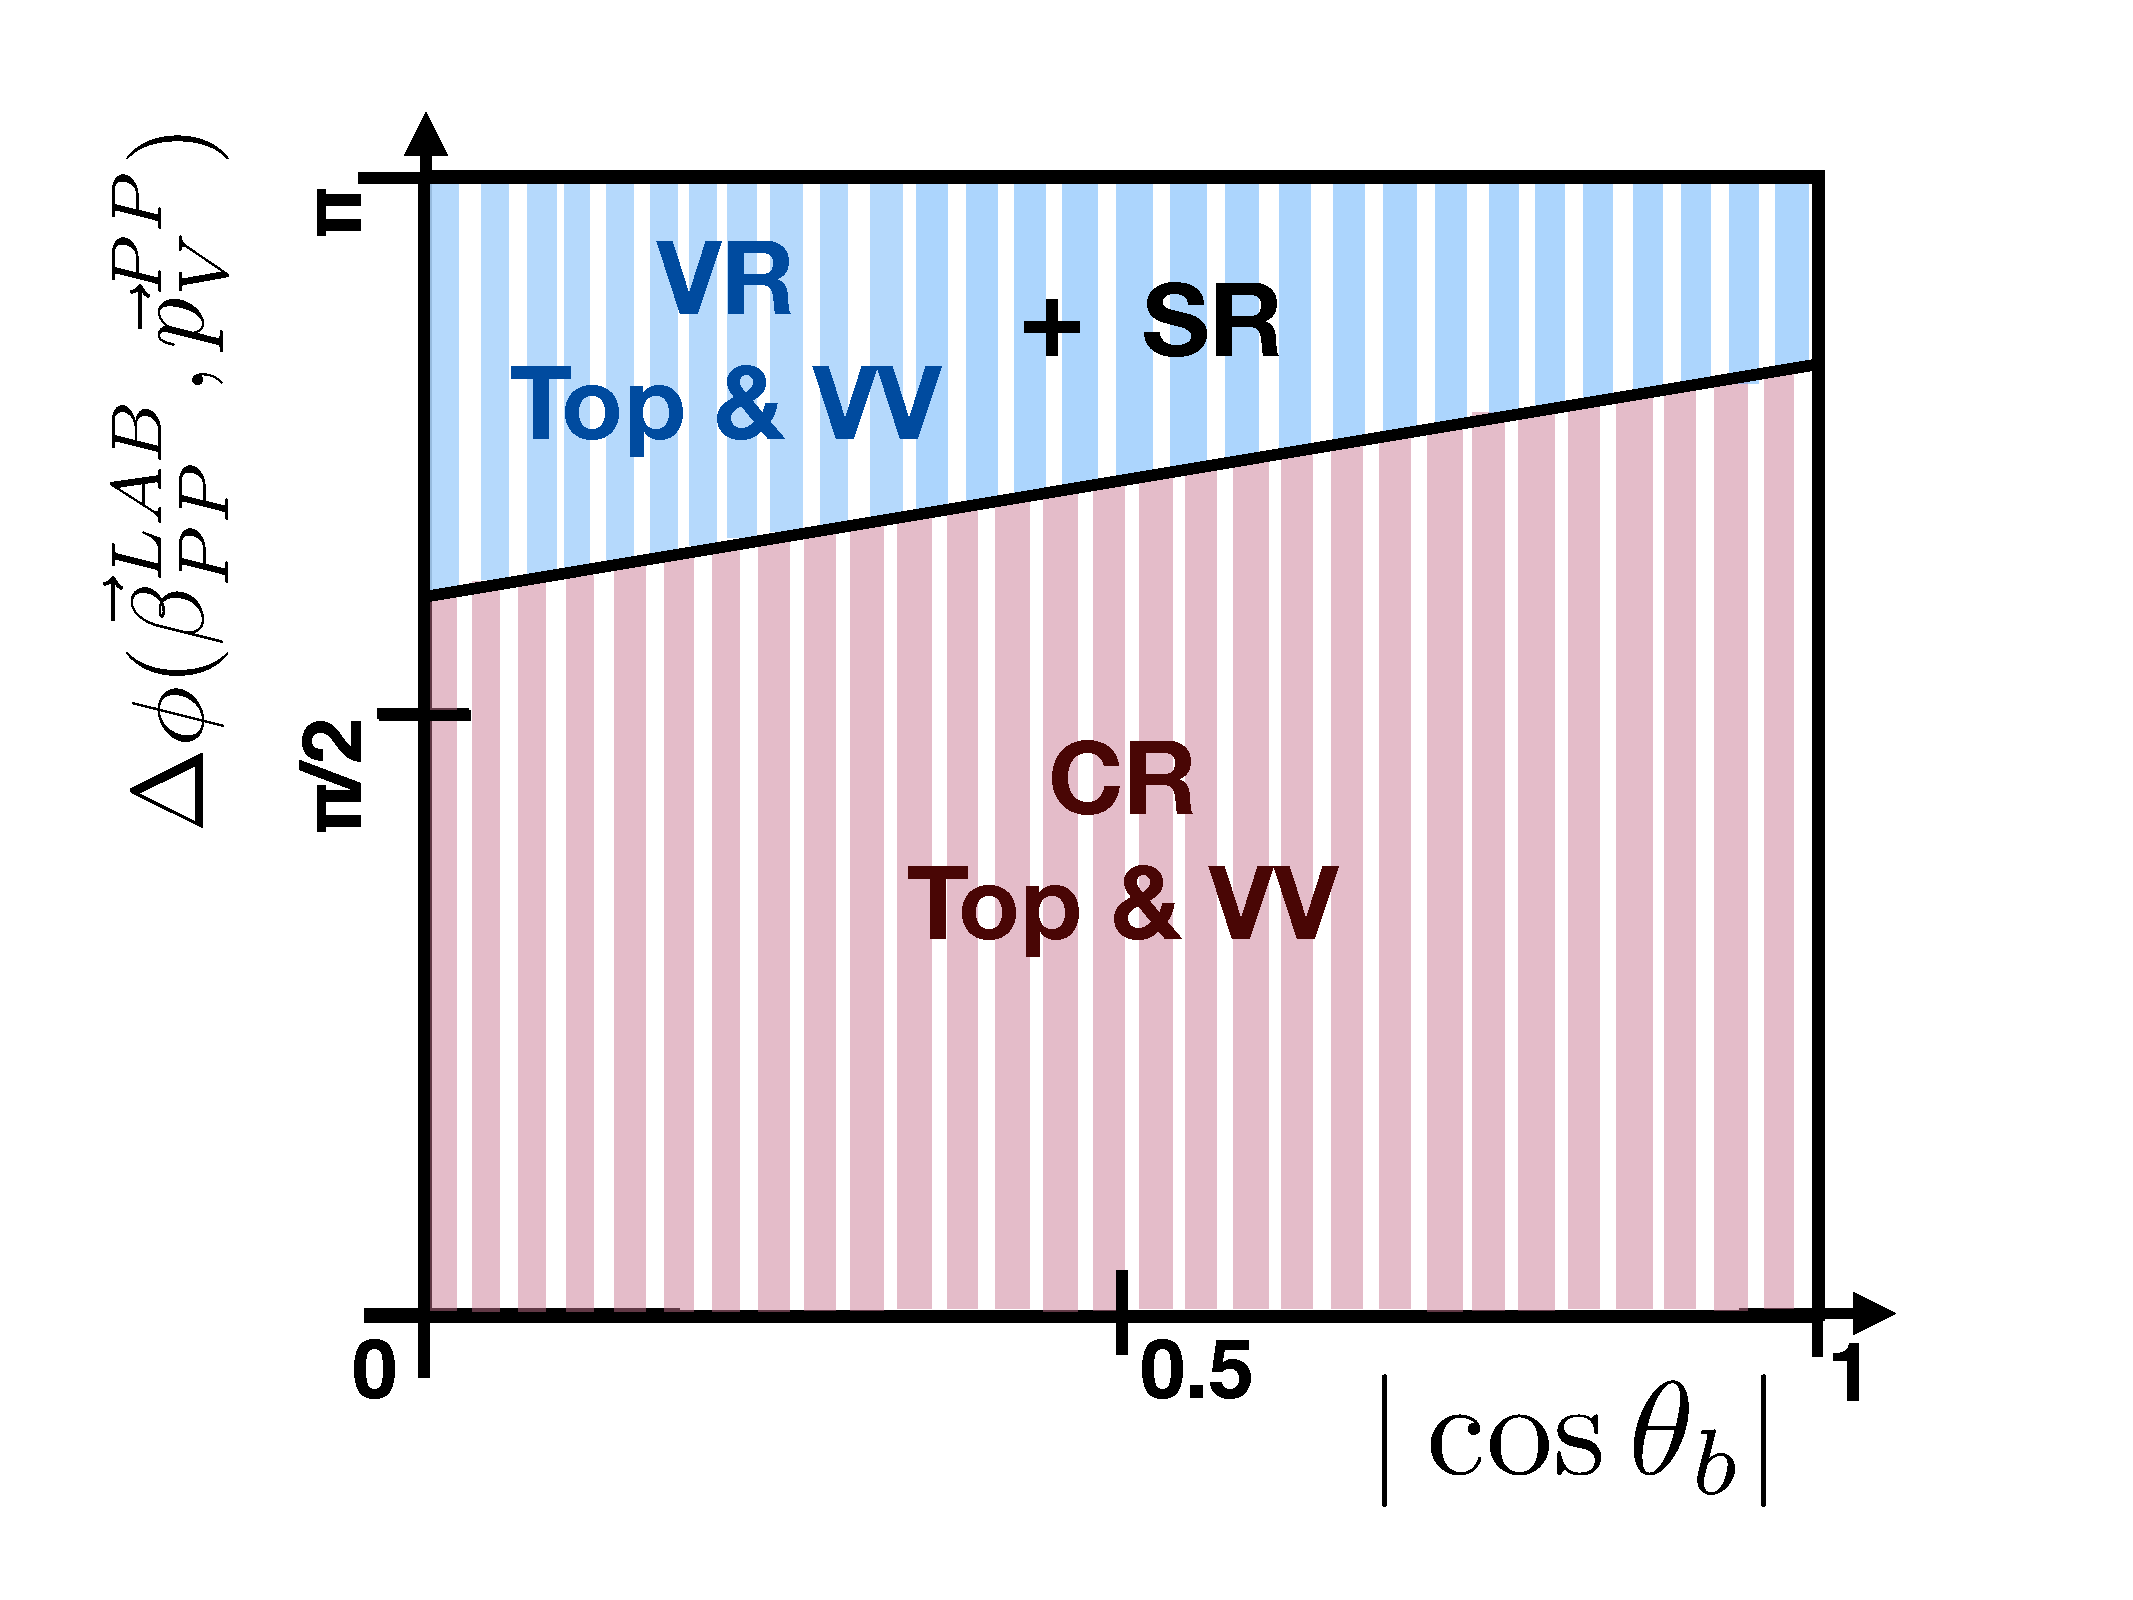
\includegraphics[width=0.7\textwidth]{figures/search_stop2l/bkg_est/crvrmotivation}
        \caption{
            Illustration of the CR and VR strategy used in the \bWN search.
            The defining characteristic for the definition of these regions is
            based on the region in the $(\cosb, \dpb)$-plane that they select.
            The CR inverts the requirements on these quantities relative to the SRs,
            while the VR has the same requirements as in the SRs but inverts
            selections made on the other observables.
        }
        \label{fig:stop_crvr_motivation}
    \end{center}
\end{figure}

%%%%%%%%%%%%%%%%%%%%%%%%%%%%%%%%%%%%%%%%%%%%%%%%%%%%%%%%%%%%%%%%%%%%%%%%%%%%%%%%%%%%%%%%%%%%
%%%%%%%%%%%%%%%%%%%%%%%%%%%%%%%%%%%%%%%%%%%%%%%%%%%%%%%%%%%%%%%%%%%%%%%%%%%%%%%%%%%%%%%%%%%%
%%%%%%%%%%%%%%%%%%%%%%%%%%%%%%%%%%%%%%%%%%%%%%%%%%%%%%%%%%%%%%%%%%%%%%%%%%%%%%%%%%%%%%%%%%%%
%
% TOP BKG
%
%%%%%%%%%%%%%%%%%%%%%%%%%%%%%%%%%%%%%%%%%%%%%%%%%%%%%%%%%%%%%%%%%%%%%%%%%%%%%%%%%%%%%%%%%%%%
%%%%%%%%%%%%%%%%%%%%%%%%%%%%%%%%%%%%%%%%%%%%%%%%%%%%%%%%%%%%%%%%%%%%%%%%%%%%%%%%%%%%%%%%%%%%
%%%%%%%%%%%%%%%%%%%%%%%%%%%%%%%%%%%%%%%%%%%%%%%%%%%%%%%%%%%%%%%%%%%%%%%%%%%%%%%%%%%%%%%%%%%%

\subsection{Top-quark pair production}
\label{sec:stop_ttbar_estimate}

\begin{table}[!htb]
    \begin{center}
        \caption{
            Definitions of the CR and VR for the \ttbar~background process for the
            \bWN search.
        }
        \begin{tabular}{l | c c}
            \hline
            \hline
                & \multicolumn{2}{c}{\textbf{Regions}} \\
            \hline
            \textbf{Variable} & \textbf{CR-Top} & \textbf{VR-Top} \\
            \hline
            Dilepton Flavor & \multicolumn{2}{c}{DF} \\
            $m_{\ell\ell}$ [GeV]    & \multicolumn{2}{c}{no req.} \\
            Lead lepton \pT [GeV] & \multicolumn{2}{c}{$>25$} \\
            Sub-lead lepton \pT [GeV] & \multicolumn{2}{c}{$>20$} \\
            $b$-tagged jet multiplicity & $>0$ & Exactly 0 \\
            \mdr [GeV] & \multicolumn{2}{c}{$>80$} \\
            \rpt & $>0.7$ & $<0.7$ \\
            \gaminv & \multicolumn{2}{c}{no req.} \\
            $(\cosb, \dpb)$ & $\dpb $ & $\dpb$ \\
                    & \hspace{1.8cm} $< 0.9 \times | \cosb | + 1.6$ & \hspace{1.8cm}$> 0.9 \times | \cosb | + 1.6$ \\
            \hline
            \hline
        \end{tabular}
    \end{center}
\end{table}



%%%%%%%%%%%%%%%%%%%%%%%%%%%%%%%%%%%%%%%%%%%%%%%%%%%%%%%%%%%%%%%%%%%%%%%%%%%%%%%%%%%%%%%%%%%%
%%%%%%%%%%%%%%%%%%%%%%%%%%%%%%%%%%%%%%%%%%%%%%%%%%%%%%%%%%%%%%%%%%%%%%%%%%%%%%%%%%%%%%%%%%%%
%%%%%%%%%%%%%%%%%%%%%%%%%%%%%%%%%%%%%%%%%%%%%%%%%%%%%%%%%%%%%%%%%%%%%%%%%%%%%%%%%%%%%%%%%%%%
%
% VV BKG
%
%%%%%%%%%%%%%%%%%%%%%%%%%%%%%%%%%%%%%%%%%%%%%%%%%%%%%%%%%%%%%%%%%%%%%%%%%%%%%%%%%%%%%%%%%%%%
%%%%%%%%%%%%%%%%%%%%%%%%%%%%%%%%%%%%%%%%%%%%%%%%%%%%%%%%%%%%%%%%%%%%%%%%%%%%%%%%%%%%%%%%%%%%
%%%%%%%%%%%%%%%%%%%%%%%%%%%%%%%%%%%%%%%%%%%%%%%%%%%%%%%%%%%%%%%%%%%%%%%%%%%%%%%%%%%%%%%%%%%%

\subsection{Diboson Production}
\label{sec:stop_vv_estimate}

\begin{table}[!htb]
    \begin{center}
        \caption{
            Definitions of the CR and VR for the diboson~background processes for the
            \bWN search.
        }
        \begin{tabular}{l | c c c c}
            \hline
            \hline
                & \multicolumn{4}{c}{\textbf{Regions}} \\
            \hline
            \textbf{Variable} & \textbf{CR-VV-DF} & \textbf{CR-VV-SF} & \textbf{VR-VV-DF} & \textbf{VR-VV-SF} \\
            \hline
            Dilepton Flavor & DF & SF & DF & SF \\
            $m_{\ell\ell}$ [GeV]    & no req. & $|m_{\ell\ell} - 91.2| > 10$ & no req. & $|m_{\ell\ell} - 91.2| > 10$ \\
            Lead lepton \pT [GeV] & $>25$ & $>25$ & $>25$ & $>25$ \\
            Sub-lead lepton \pT [GeV] & $>20$ & $>20$ & $>20$ & $>20$ \\
            $b$-tagged jet multiplicity & Exactly 0 & Exactly 0 & Exactly 0 & Exactly 0 \\
            \mdr [GeV] & $>50$ & $>70$ & $\in(50,95)$ & $\in(60,95)$ \\
            \rpt & $<0.5$ & $<0.5$ & $<0.7$ & $<0.4$ \\
            \gaminv &  $>0.7$ & $>0.7$ & $>0.7$ & $>0.7$ \\
            $(\cosb, \dpb)$ & \multicolumn{2}{c}{\small{$\dpb < 0.9 \times | \cosb | + 1.6$}} & \multicolumn{2}{c}{\small{$\dpb> 0.9 \times | \cosb | + 1.6$}} \\
%            $(\cosb, \dpb)$ & $\dpb $  &  $\dpb$ & \\
%                    & \hspace{1.8cm} $< 0.9 \times | \cosb | + 1.6$  & \hspace{1.8cm}$> 0.9 \times | \cosb | + 1.6$ \\
            \hline
            \hline
        \end{tabular}
    \end{center}
\end{table}

%%%%%%%%%%%%%%%%%%%%%%%%%%%%%%%%%%%%%%%%%%%%%%%%%%%%%%%%%%%%%%%%%%%%%%%%%%%%%%%%%%%%%%%%%%%%
%%%%%%%%%%%%%%%%%%%%%%%%%%%%%%%%%%%%%%%%%%%%%%%%%%%%%%%%%%%%%%%%%%%%%%%%%%%%%%%%%%%%%%%%%%%%
%%%%%%%%%%%%%%%%%%%%%%%%%%%%%%%%%%%%%%%%%%%%%%%%%%%%%%%%%%%%%%%%%%%%%%%%%%%%%%%%%%%%%%%%%%%%
%
% POST FIT
%
%%%%%%%%%%%%%%%%%%%%%%%%%%%%%%%%%%%%%%%%%%%%%%%%%%%%%%%%%%%%%%%%%%%%%%%%%%%%%%%%%%%%%%%%%%%%
%%%%%%%%%%%%%%%%%%%%%%%%%%%%%%%%%%%%%%%%%%%%%%%%%%%%%%%%%%%%%%%%%%%%%%%%%%%%%%%%%%%%%%%%%%%%
%%%%%%%%%%%%%%%%%%%%%%%%%%%%%%%%%%%%%%%%%%%%%%%%%%%%%%%%%%%%%%%%%%%%%%%%%%%%%%%%%%%%%%%%%%%%

\begin{table}[!htb]
\begin{center}
\setlength{\tabcolsep}{0.0pc}
{\scriptsize
\caption{
Yields in the \ttbar~and diboson CRs and VRs for the \bWN search for the main background processes
contributing to the analysis.
The lower-portion of the table are the yields before the background-only fit to data
in the CRs, without the normalisation corrections applied.
The upper-portion of the table are those taken after the background-only fit to data.
The errors on the quoted numbers are due to the statistical and experimental systematic uncertainties.
}
\label{tab:bkgonly_CRVR}
\begin{tabular*}{\textwidth}{@{\extracolsep{\fill}}lrrrrrr}
\noalign{\smallskip}\hline\noalign{\smallskip}
\noalign{\smallskip}\hline\noalign{\smallskip}
\textbf{Process}           & \textbf{CR-Top}            & \textbf{CR-VV-DF}            & \textbf{CR-VV-SF}            & \textbf{VR-Top}           & \textbf{VR-VV-DF}            & \textbf{VR-VV-SF}              \\[-0.05cm]
\noalign{\smallskip}\hline\noalign{\smallskip}


Observed Data         & $951$              & $2046$              & $1275$              & $1197$              & $1896$              & $783$                    \\
\noalign{\smallskip}\hline\noalign{\smallskip}
%%
Post-fit Total SM         & $951.00 \pm 30.84$          & $2046.05 \pm 45.23$          & $1275.17 \pm 35.68$          & $1231.78 \pm 86.59$          & $2013.57 \pm 116.49$          & $780.44 \pm 117.32$              \\
\noalign{\smallskip}\hline\noalign{\smallskip}
%%
        Post-fit \ttbar          & $833.03 \pm 32.85$          & $619.74 \pm 111.40$          & $333.62 \pm 60.91$          & $733.87 \pm 64.91$          & $754.94 \pm 78.17$          & $127.14 \pm 22.09$              \\
%%
        Post-fit Diboson (DF)          & $11.51 \pm 2.43$          & $1093.28 \pm 125.83$          & $0.00 \pm 0.00$          & $331.13 \pm 82.57$          & $886.53 \pm 168.16$          & $0.00 \pm 0.00$              \\
%%
        Post-fit Diboson (SF)          & $0.00 \pm 0.00$          & $0.00 \pm 0.00$          & $378.94 \pm 124.32$          & $0.00 \pm 0.00$          & $0.00 \pm 0.00$          & $380.00 \pm 141.58$              \\
%%
        Post-fit Single-top          & $101.10 \pm 9.73$          & $186.47 \pm 27.99$          & $103.47 \pm 17.43$          & $111.52 \pm 14.49$          & $151.88 \pm 14.37$          & $36.40 \pm 5.62$              \\
%%
        Post-fit $\ttbar+V$          & $4.35 \pm 0.42$          & $0.39 \pm 0.07$          & $0.36 \pm 0.07$          & $1.27 \pm 0.22$          & $0.42 \pm 0.13$          & $0.05 \pm 0.02$              \\
%%
        Post-fit $Z$+jets          & $0.70 \pm 0.22$          & $1.83_{-1.83}^{+2.55}$          & $428.58 \pm 92.55$          & $0.47_{-0.47}^{+0.85}$          & $0.39_{-0.39}^{+0.71}$          & $191.37 \pm 78.38$              \\
%%
        Post-fit Single-higgs          & $0.31 \pm 0.13$          & $78.95 \pm 9.17$          & $6.23 \pm 1.06$          & $0.44_{-0.44}^{+0.52}$          & $54.98 \pm 4.34$          & $9.40 \pm 1.11$              \\
%%
        Post-fit Fakes          & $0.00 \pm 0.00$          & $65.37 \pm 2.22$          & $23.96 \pm 1.25$          & $53.09 \pm 1.92$          & $164.42 \pm 5.68$          & $36.09 \pm 3.04$              \\
%%
 \noalign{\smallskip}\hline\noalign{\smallskip}
%%
 Total SM               & $905.14 \pm 16.54$          & $1988.38 \pm 110.43$          & $1248.21 \pm 123.42$          & $1184.39 \pm 71.23$          & $1952.92 \pm 61.72$          & $764.65 \pm 99.06$              \\
\noalign{\smallskip}\hline\noalign{\smallskip}
%%
         \ttbar          & $787.43 \pm 11.29$          & $585.87 \pm 102.00$          & $315.39 \pm 55.87$          & $693.71 \pm 53.51$          & $713.64 \pm 66.57$          & $120.19 \pm 20.17$              \\
%%
         Diboson (DF)          & $11.25 \pm 1.62$          & $1069.46 \pm 12.45$          & $0.00 \pm 0.00$          & $323.89 \pm 50.27$          & $867.18 \pm 77.75$          & $0.00 \pm 0.00$              \\
%%
         Diboson (SF)          & $0.00 \pm 0.00$          & $0.00 \pm 0.00$          & $370.13 \pm 15.48$          & $0.00 \pm 0.00$          & $0.00 \pm 0.00$          & $371.16 \pm 34.38$              \\
%%
         Single-top          & $101.10 \pm 9.80$          & $186.49 \pm 28.25$          & $103.49 \pm 17.59$          & $111.52 \pm 14.60$          & $151.88 \pm 14.46$          & $36.41 \pm 5.66$              \\
%%
         $\ttbar+V$          & $4.35 \pm 0.42$          & $0.39 \pm 0.07$          & $0.36 \pm 0.07$          & $1.27 \pm 0.23$          & $0.42 \pm 0.13$          & $0.05 \pm 0.02$              \\
%%
         $Z$+jets          & $0.70 \pm 0.23$          & $1.83_{-1.83}^{+2.57}$          & $428.65 \pm 93.15$          & $0.48_{-0.48}^{+0.86}$          & $0.40_{-0.40}^{+0.72}$          & $191.36 \pm 78.78$              \\
%%
         Single-higgs          & $0.31 \pm 0.13$          & $78.96 \pm 9.26$          & $6.23 \pm 1.07$          & $0.44_{-0.44}^{+0.53}$          & $54.98 \pm 4.37$          & $9.40 \pm 1.12$              \\
%%
         Fakes          & $0.00 \pm 0.00$          & $65.37 \pm 2.23$          & $23.96 \pm 1.26$          & $53.09 \pm 1.92$          & $164.42 \pm 5.70$          & $36.09 \pm 3.04$              \\
\noalign{\smallskip}\hline\noalign{\smallskip}
\noalign{\smallskip}\hline\noalign{\smallskip}
\end{tabular*}
}
\end{center}
\end{table}
